\documentclass[article, 12pt, 3p]{elsarticle}

\usepackage{natbib} 
\setcitestyle{authoryear,open={(},close={)}}
%\bibliographystyle{plainnat}

\usepackage{etoolbox,comment,setspace,fancyhdr,hyperref,color,graphicx,subcaption,booktabs,rotating,multirow}

\captionsetup[subfigure]{labelformat=simple,labelsep=space}
\renewcommand\thesubfigure{(\roman{subfigure})}

\newcounter{rowfig}
\renewcommand{\therowfig}{\Alph{rowfig}}

\usepackage{amsmath,amsthm,amssymb,amstext,bbold,amsfonts}
\usepackage{float,caption}
\usepackage{threeparttable}
\usepackage{lscape}
\usepackage{bbm}
\usepackage{adjustbox}
\usepackage[tracking=true]{microtype}
%\usepackage[pdftex, letterpaper, margin=1in, headheight=-.25cm]{geometry}
 %\usepackage[abbr]{harvard}
 
\hypersetup{
  colorlinks   = true, %Colours links instead of ug dly boxes
  urlcolor     = blue, %Colour for external hyperlinks
  linkcolor    = black, %Colour of internal links 
  citecolor   = blue %Colour of citations
}

\newtheorem{proposition}{Proposition}
\newtheorem{definition}{Definition}
\newtheorem{assumption}{Assumption}
\newtheorem{condition}{Condition}
\newtheorem{lemma}{Lemma}
\newtheorem{conjecture}{Conjecture}
\newtheorem{corollary}{Corollary}
\numberwithin{corollary}{proposition}
%\numberwithin{equation}{section}
% [[prompt01]] original: \numberwithin{equation}{}

%\newcommand{\inv}{\makebox[0pt][l]{$^{-1}$}}
\pdfoptionpdfminorversion=6 

%Define argmax
\DeclareMathOperator*{\argmax}{arg\,max}

%%Put space between captions and figures.
%\setlength{\belowcaptionskip}{6pt}

\makeatletter
\def\ps@pprintTitle{%
   \let\@oddhead\@empty
   \let\@evenhead\@empty
   \let\@oddfoot\@empty
   \let\@evenfoot\@oddfoot
}
\makeatother
\usepackage{ragged2e}
\usepackage{setspace} 
\usepackage{caption}
% [[prompt01]] original: \usepackage[usenames,dvipsnames]{pstricks}
% [[prompt01]] original: \usepackage{epsfig}
% [[prompt01]] original: \usepackage{pst-grad} % For gradients
% [[prompt01]] original: \usepackage{pst-plot} % For axes
 \usepackage[space]{grffile} % For spaces in paths
 \makeatletter % For spaces in paths
 \patchcmd\Gread@eps{\@inputcheck#1 }{\@inputcheck"#1"\relax}{}{}
 \makeatother
\usepackage[utf8]{inputenc}
% [[prompt01]] original: \usepackage{stackrel}
\IfFileExists{stackrel.sty}{\usepackage{stackrel}}{}
\usepackage{array}
\usepackage{siunitx}
% [[prompt02]] added: column-width convention of the reference (_reference_productivity/Tables/_tabledefs.tex,
% copied, not \input): N{<width>} centred numeric column, L{<width>} ragged-right label column.
\usepackage{makecell}
\newcolumntype{N}[1]{>{\centering\arraybackslash}p{#1}}
\newcolumntype{L}[1]{>{\raggedright\arraybackslash}p{#1}}
\newlength{\labelw}\setlength{\labelw}{0.22\textwidth}
\newlength{\labelwwide}\setlength{\labelwwide}{0.36\textwidth}
\newlength{\labelwnarrow}\setlength{\labelwnarrow}{0.19\textwidth}
\newcommand{\colwfor}[2]{\dimexpr(\textwidth-(#2)-\tabcolsep*\numexpr2*#1+2\relax)/#1\relax}
\newcommand{\colwform}[3]{\dimexpr(\textwidth-(#3)-\tabcolsep*\numexpr2*#1+2*#2\relax)/#1\relax}
\newcommand{\colw}{\colwfor{6}{\labelw}}
\newcommand{\colwvii}{\colwfor{7}{\labelw}}
\newcommand{\colwnarrow}{\colwfor{8}{\labelw}}
\newcommand{\notesize}{\footnotesize}
\setlength{\extrarowheight}{4pt}
\renewcommand\normalsize{\fontsize{11}{8}\selectfont}
\newcommand\narrowstyle{\SetTracking{encoding=*}{-10}\lsstyle}
\newcommand\vnarrowstyle{\SetTracking{encoding=*}{-40}\lsstyle}
\newcommand\vvnarrowstyle{\SetTracking{encoding=*}{-75}\lsstyle}

\newcommand\narrowtext[1]{\textls[-10]{#1}}
\newcommand\vnarrowtext[1]{\textls[-40]{#1}}
\newcommand\vvnarrowtext[1]{\textls[-75]{#1}}

\makeatletter
\renewcommand\footnotesize{%
   \@setfontsize\footnotesize\@ixpt{9}%
   \abovedisplayskip 8\p@ \@plus2\p@ \@minus4\p@
   \abovedisplayshortskip \z@ \@plus\p@
   \belowdisplayshortskip 4\p@ \@plus2\p@ \@minus2\p@
   \def\@listi{\leftmargin\leftmargini
               \topsep 4\p@ \@plus2\p@ \@minus2\p@
               \parsep 2\p@ \@plus\p@ \@minus\p@
               \itemsep \parsep}%
   \belowdisplayskip \abovedisplayskip
}
\makeatother

\usepackage{setspace}
\usepackage[T1]{fontenc}
\usepackage{array}
\usepackage{longtable}
\usepackage{pdfpages}
\usepackage{dsfont}
\newcommand{\bc}{\begin{center}}
\newcommand{\ec}{\end{center}}
\newcommand{\bt}{\begin{tabular}}
\newcommand{\et}{\end{tabular}}
\newcommand{\bi}{\begin{itemize}}
\newcommand{\ei}{\end{itemize}}
\newcommand{\ben}{\begin{enumerate}}
\newcommand{\een}{\end{enumerate}}
\newcommand{\bd}{\begin{displaymath}}
\newcommand{\ed}{\end{displaymath}}
\newcommand{\beann}{\begin{eqnarray*}}
\newcommand{\eeann}{\end{eqnarray*}}
\newcommand{\bea}{\begin{eqnarray}}
\newcommand{\eea}{\end{eqnarray}}
\newcommand{\ba}{\begin{array}}
\newcommand{\ea}{\end{array}}
\newcommand{\bma}{\begin{pmatrix}}
\newcommand{\ema}{\end{pmatrix}}
%}}}
%Math Shortcuts {{{
\newcommand{\Ra}{\Rightarrow}
\newcommand{\bbR}{\mathbb{R}}
\newcommand{\bbY}{\mathbb{Y}}
\newcommand{\bbF}{\mathbb{F}}
\newcommand{\bbS}{\mathbb{S}}
\newcommand{\bbN}{\mathbb{N}}
\newcommand{\bbG}{\mathbb{G}}
\newcommand{\bbT}{\mathbb{T}}
\newcommand{\deB}{\mathcal{B}}
\newcommand{\deW}{\mathcal{W}}
\newcommand{\deR}{\mathcal{R}}
\newcommand{\deF}{\mathcal{F}}
\newcommand{\deA}{\mathcal{A}}
\newcommand{\deY}{\mathcal{Y}}
\newcommand{\deS}{\mathcal{S}}
\newcommand{\deL}{\mathcal{L}}
\newcommand{\deH}{\mathcal{H}}
\newcommand{\deE}{\mathcal{E}}
\newcommand{\deP}{\mathcal{P}}
\newcommand{\deG}{\mathcal{G}}
\newcommand{\deT}{\mathcal{T}}
\newcommand{\deff}{\mathcal{f}}
\newcommand{\dep}{\mathcal{p}}
\newcommand{\E}{\mathnormal{E}}
\newcommand{\var}{\mathnormal{V\!AR}}
\newcommand{\Cov}{\mathnormal{COV}}
\newcommand{\Corr}{\mathnormal{CORR}}
\newcommand{\Prob}{\mathnormal{Prob}}
%}}}
%Additional Shortcuts {{{
\newcommand{\mD}{\displaystyle}
\newcommand{\mT}{\textstyle}
\newcommand{\mS}{\scriptstyle}
\newcommand{\mSS}{\scriptscriptstyle}
\newcommand{\m}[1]{\,#1\,}
\newcommand{\nn}{\nonumber}
\newcommand{\colorEmphText}{\color{blue}}
\newcommand{\colorEmphBackground}{\color{yellow}}
%}}}
% \usepackage[stable]{footmisc} 
\newcommand*{\mycommand}[1]{\texttt{\emph{#1}}}
% [[prompt01]] original: \renewcommand*{\thefootnote}{\fnsymbol{footnote}}
%% these three are essential for estout
\usepackage{booktabs}  % neatly formatting lines
\usepackage{threeparttable}    
\usepackage{dcolumn}    % aligning decimals
    \newcolumntype{d}[1]{D{.}{.}{#1}}
% Estout LaTeX wrapper (by Jörg Weber)
\let\estinput=\input % define a new input command so that we can still flatten the document
\newcommand{\estwide}[3]{
		\vspace{.75ex}{
			%\textsymbols% Note the added command here
			\begin{tabular*}
			{\textwidth}{@{\hskip\tabcolsep\extracolsep\fill}l*{#2}{#3}}
			\toprule
			\estinput{#1}
			\addlinespace[.75ex]
			\end{tabular*}
			}
		}	
\newcommand{\estauto}[3]{
		\vspace{.75ex}{
			%\textsymbols% Note the added command here
			\begin{tabular}{l*{#2}{#3}}
			\toprule
			\estinput{#1}
			\\ \bottomrule           % 08 Dec 2021. Add these slashes.
			\addlinespace[-.75]
			\end{tabular}
			}
		}
% Allow line breaks with \\ in specialcells
\newcommand{\specialcell}[2][c]{%
    \begin{tabular}[#1]{@{}c@{}}#2\end{tabular}
}
\usepackage{float}
\usepackage[section]{placeins}
% [[prompt02d]] floats share pages with text instead of going to float pages
\renewcommand{\topfraction}{0.9}
\renewcommand{\bottomfraction}{0.8}
\renewcommand{\textfraction}{0.07}
\renewcommand{\floatpagefraction}{0.85}
\setcounter{topnumber}{3}
\setcounter{bottomnumber}{2}
\setcounter{totalnumber}{4}
\setlength{\floatsep}{10pt plus 2pt minus 2pt}
\setlength{\textfloatsep}{14pt plus 2pt minus 2pt}
\setlength{\intextsep}{12pt plus 2pt minus 2pt}
\newcommand{\sym}[1]{\rlap{#1}}% Thanks David Carlisle
\usepackage{hhline}
\captionsetup{font=normalsize} 


 % Note/Source/Text after Tables
\newcommand{\figtext}[1]{
	\vspace{-1.9ex}
	\captionsetup{justification=justified,font=scriptsize}
	\caption*{\hspace{6pt}\hangindent=1.5em #1}
	} 
\newcommand{\fignote}[1]{\figtext{\emph{Note:~}~#1}}

\newcommand{\figsource}[1]{\figtext{\emph{Source:~}~#1}}

% Add significance note with \starnote
\newcommand{\starnote}{\figtext{* p < 0.1, ** p < 0.05, *** p < 0.01. Standard errors in parentheses.}}
% [[prompt01]] added: source note of every table and figure (wording from main.tex l. 16)
% [[prompt02]] original: \newcommand{\srcnote}{\textit{Source:} Authors' calculations based on customs data matched to Orbis and Dun \& Bradstreet.}
\newcommand{\srcnote}{\textit{Source:} Authors' calculations based on customs data matched to Orbis (Bureau van Dijk) and Dun \& Bradstreet.}
%\usepackage{etoolbox} % to hook into `figure` and reset the mysubfig counter

% [[prompt01]] original: \usepackage{subfig}


% Checkmarks
\usepackage{tikz}
\newcommand{\tikzxmark}{%
\tikz[scale=0.23] {
    \draw[line width=0.7,line cap=round] (0,0) to [bend left=6] (1,1);
    \draw[line width=0.7,line cap=round] (0.2,0.95) to [bend right=3] (0.8,0.05);
}}
\newcommand{\tikzcmark}{% 
\tikz[scale=0.23] {
    \draw[line width=0.7,line cap=round] (0.25,0) to [bend left=10] (1,1);
    \draw[line width=0.8,line cap=round] (0,0.35) to [bend right=1] (0.23,0);
}}
%\renewcommand{\arraystretch}{0.9}
% [[prompt02]] original: \renewcommand{\arraystretch}{0.8}
% [[prompt02]] original: \setlength{\tabcolsep}{5pt}
 \makeatletter
\newcommand*\mysize{%
  \@setfontsize\mysize{7.5}{9.0}%
}

\makeatother
% For reference:
%\[
%    \checkmark
%    \tikzxmark
%    \tikzcmark
%\]

%\onehalfspacing

% [[prompt03b]] elsarticle draws two rules around the (absent) abstract; suppress them for this summary
\makeatletter
\let\els@maketitle\maketitle
\renewcommand{\maketitle}{\begingroup\let\hrule\relax\els@maketitle\endgroup}
\makeatother
\begin{document}

\title{$\,$\\ $\,$\\ $\,$\\\vspace{-4.9em}\LARGE\textbf{Multinational Firms and Agricultural Trade in Latin America}\footnote{The views and interpretations in this paper are strictly those of the authors and should not be attributed to the Inter-American Development Bank, its executive directors, or its member countries.}}
\author{\vskip 2em This version: October 2026\\[2pt] \small Preliminary draft, please do not circulate}

\thispagestyle{empty}
\maketitle
\setcounter{page}{0}\setcounter{footnote}{0}
\renewcommand\normalsize{\fontsize{12}{20}\selectfont}\normalsize
\newpage

\section{Data}

The data come from two sources. The first is the export transactions recorded by the customs agencies of nine Latin
American countries: Argentina, Chile, Colombia, Costa Rica, the Dominican Republic, El Salvador, Paraguay, Peru and
Uruguay. For each export, they report the exporting firm, the product at the six-digit level of the Harmonized System,
the destination, the year and the value. The period is 2012--2018, the years in which all nine countries are observed,
and agricultural products are chapters 01 to 24 of the Harmonized System. The second source is ownership data from
Orbis, compiled by Bureau van Dijk, and Dun \& Bradstreet, which report each company's global ultimate owner and its
country. Exporters are linked to these records by tax identifiers, by name matching confirmed with a large language
model, and by a manual review of the largest unmatched exporters. The country of the parent is known for 89 percent of
the agricultural exports of foreign affiliates.

Exporters linked to the ownership data are affiliates of multinational firms (MNEs): domestic when the ultimate parent is located in the exporting country, foreign otherwise. Exporters that cannot be linked are local firms, which we also refer to as non-MNE firms. In 2018, 12,993
firms exported 875 agricultural products to 211 countries, for a total of US\$78.5 billion. Agriculture accounts for
35 percent of the merchandise exports of the nine countries, with wide differences across them: 84 percent in
Paraguay, 56 percent in Argentina and 52 percent in Uruguay, and between 17 and 24 percent in Colombia, El Salvador,
Peru, the Dominican Republic and Chile. Argentina alone ships 44 percent of the region's agricultural exports.

\section{Stylized facts}

Six stylized facts summarize the data; the first three describe 2018, the last three come from regressions on
2012--2018.

\subsection{Fact 1: Multinationals ship almost half of agricultural exports}

Multinational firms ship almost half of agricultural exports. In 2018 they shipped 47.5 percent, 39.6 percent through
foreign affiliates and 7.9 percent through domestic ones (Figure~\ref{fig:f1}, Panel A); these exports come from 3,181
affiliates of 1,908 multinational groups whose parents are based in 112 countries. The share is highest in Uruguay (72
percent) and Paraguay (69 percent) and lowest in El Salvador (30 percent), Colombia (40 percent) and Peru (40
percent), and the parents behind these shares differ across countries (Panel B).

% ---- Figure: Multinational share of agricultural exports, by exporting country, 2018
\begin{figure}[htbp]
\centering
\caption{Multinational share of agricultural exports, by exporting country, 2018}
\label{fig:f1}
{\small\textit{Panel A. Foreign and domestic multinationals}}\par\vspace{1pt}
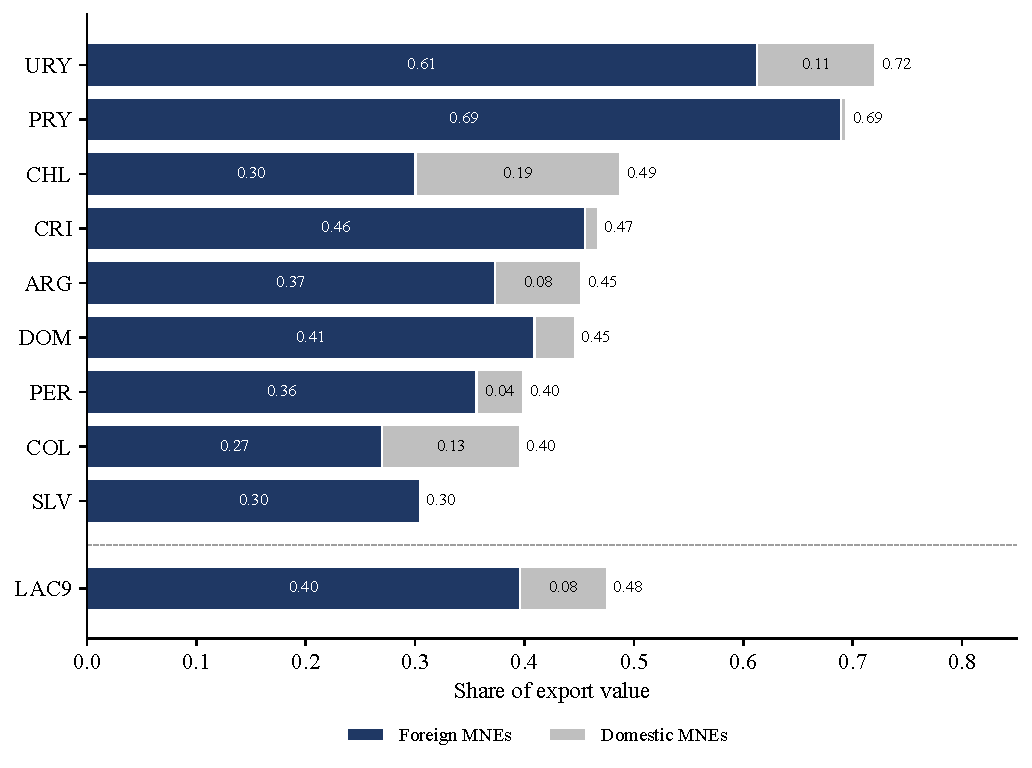
\includegraphics[width=0.72\textwidth,height=0.30\textheight,keepaspectratio]{figures/agro2018/fig_agp_origin_lac9.pdf}
\par\vspace{3pt}
{\small\textit{Panel B. Multinationals by parent country}}\par\vspace{1pt}
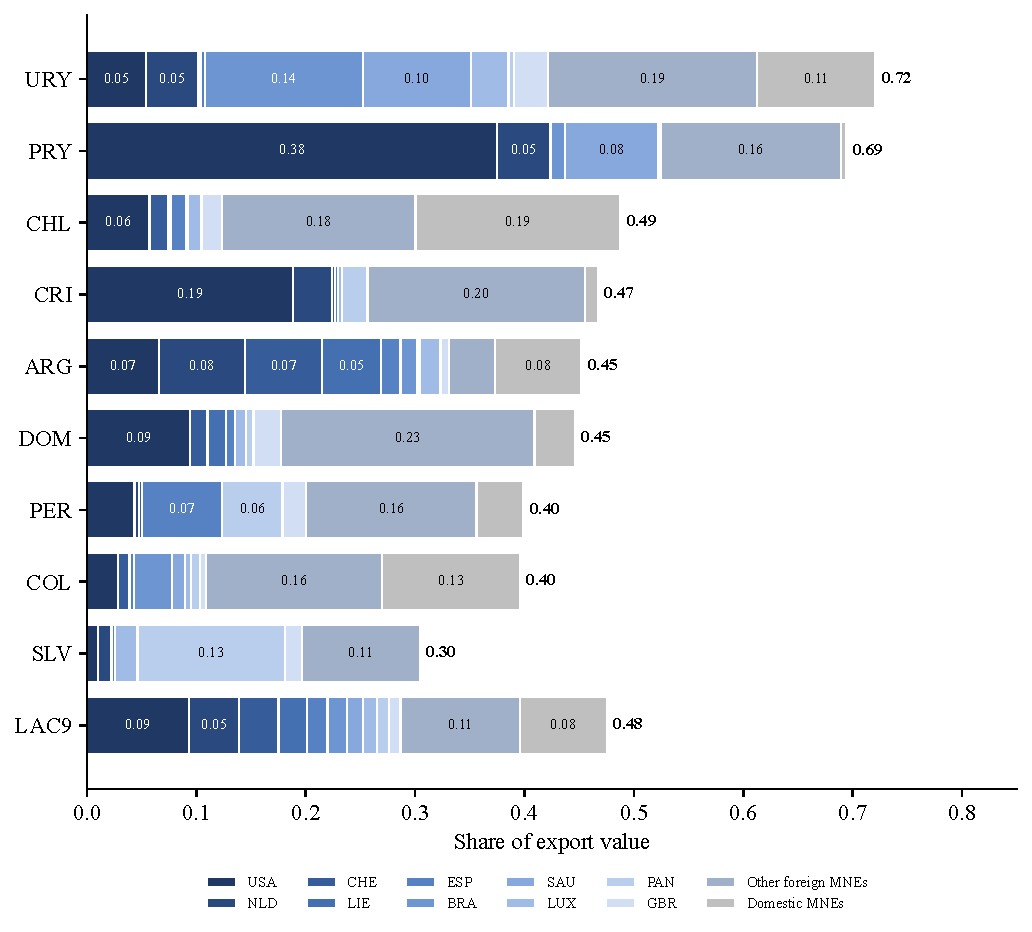
\includegraphics[width=0.85\textwidth,height=0.32\textheight,keepaspectratio]{figures/agro2018/fig_wp1a_origin_by_parent_lac9.pdf}

\begin{minipage}{0.9\linewidth}
\notesize
\vspace{0.6em}
\textit{Notes:} Shares of agricultural export value (HS 01--24) in 2018. Panel A: LAC9 is the nine countries together; the number at the end of each bar is the total MNE share. Panel B: LAC9 at the bottom; the foreign share split among the ten largest parent countries and all other foreign parents (including matched firms with no recorded parent country); domestic MNEs have their parent in the exporting country.\\
\srcnote
\end{minipage}
\end{figure}

\FloatBarrier
\subsection{Fact 2: Parents are based in a few countries}

Parents are based in a few countries (Figure~\ref{fig:parents}). In 2018, US groups shipped 24 percent of the
agricultural exports of foreign affiliates and Dutch groups 12 percent, followed by groups whose parent is recorded in
Switzerland (9 percent) and Liechtenstein (7 percent); Spanish and Brazilian groups ship about 5 percent each and
Saudi groups 4 percent. Over 2012--2018, 4.5 percent of the agricultural exports of foreign affiliates went to the
country of their parent.

% ---- Figure: Foreign-multinational agricultural exports, by parent country, 2018
\begin{figure}[htbp]
\centering
\caption{Foreign-multinational agricultural exports, by parent country, 2018}
\label{fig:parents}
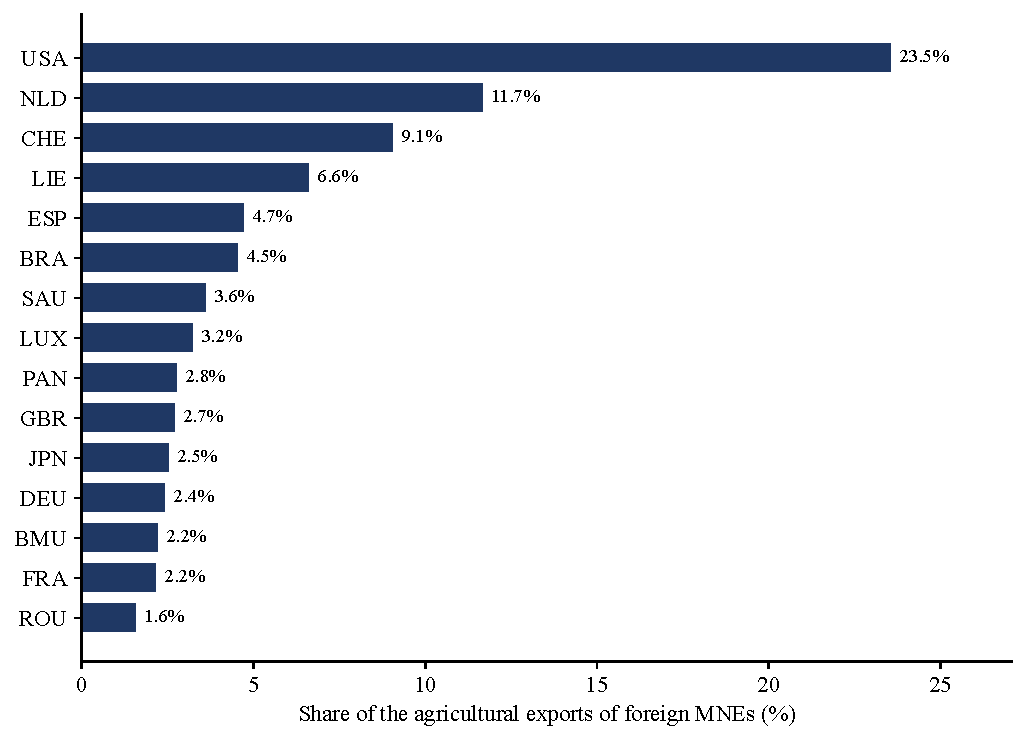
\includegraphics[width=0.78\linewidth,height=0.42\textheight,keepaspectratio]{figures/agro2018/fig_agp_parent_all.pdf}

\begin{minipage}{0.9\linewidth}
\notesize
\vspace{0.6em}
\textit{Notes:} Percent of the agricultural exports of foreign MNEs with a recorded parent country (88 percent of the total) in 2018, by country of the ultimate parent. The fifteen largest parent countries.\\
\srcnote
\end{minipage}
\end{figure}

\FloatBarrier
\subsection{Fact 3: A few large groups ship most foreign-affiliate exports}

A few large groups ship most foreign-affiliate exports (Figure~\ref{fig:network}). In 2018, 41 percent of parents had
only one affiliate in the world, but the 15 percent with more than 100 affiliates shipped 49 percent of the exports of
foreign affiliates, and groups with more than ten affiliates account for 79 percent of the total.

% ---- Figure: Foreign-multinational agricultural exports and number of parents, by size of the group's global network, 2018
\begin{figure}[htbp]
\centering
\caption{Foreign-multinational agricultural exports and number of parents, by size of the group's global network, 2018}
\label{fig:network}
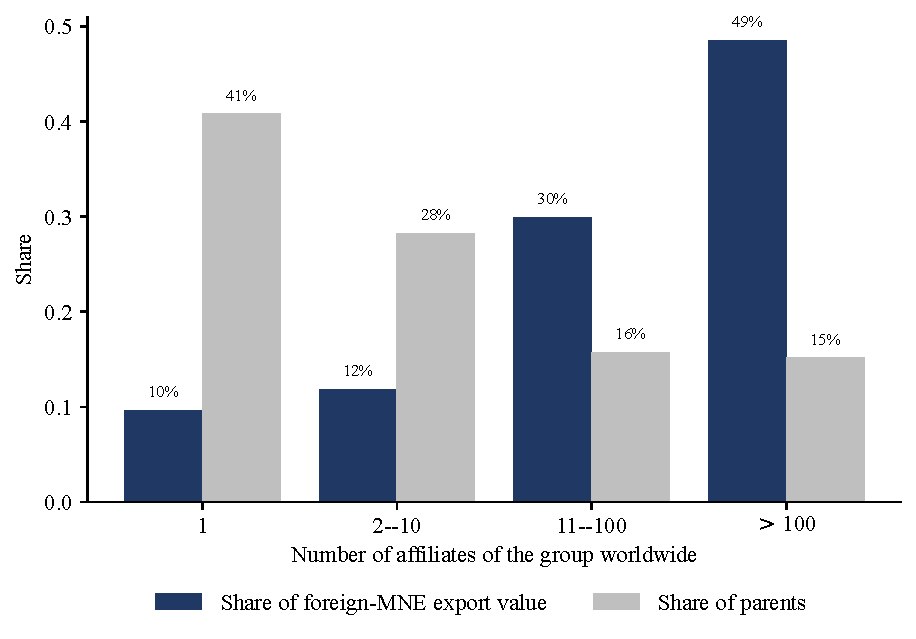
\includegraphics[width=0.78\linewidth,height=0.42\textheight,keepaspectratio]{figures/agro2018/fig_wp0_fig5_network.pdf}

\begin{minipage}{0.9\linewidth}
\notesize
\vspace{0.6em}
\textit{Notes:} Shares of foreign-MNE agricultural export value and of parents in 2018, by the number of affiliates the group has worldwide.\\
\srcnote
\end{minipage}
\end{figure}

\FloatBarrier
\subsection{Fact 4: Exports are larger where more multinationals are present}

Exports are larger where more multinational firms are present, and so are the exports of local firms
(Table~\ref{tab:t1}). In regressions at the origin--destination--product--year level with origin--destination--product
and origin--destination--year fixed effects, a 10 percent higher number of multinationals is associated with about 8
percent higher exports, and at least one multinational with exports about 90 percent higher (columns 2 and 5); for local firms, the elasticity is 0.37, and their exports are 27 percent higher when at least one multinational is present (Panel B). With the strictest fixed
effects the association is smaller but still positive and significant: 0.54 for total exports and 0.16 for local firms
(columns 3 and 6). These estimates are conditional correlations.

% ---- Table: Multinational presence and agricultural exports
\begin{table}[htbp]
\centering
\caption{Multinational presence and agricultural exports}
\label{tab:t1}
{\footnotesize\setlength{\tabcolsep}{4pt}\setlength{\extrarowheight}{1pt}
\input{tables/agro/reg_agp_presence_fx2}}

\begin{minipage}{0.95\linewidth}
\notesize
\vspace{0.6em}
\textit{Notes:} Regression at the origin country, destination country, product and year level; agricultural products, 2012--2018. Dependent variable: $\ln$ exports (Panel A) and $\ln$ exports of non-MNE firms (Panel B). Columns 1--3: $\ln$ number of MNEs, observations with at least one MNE. Columns 4--6: indicator for at least one MNE. Panel B uses only the exports of non-MNE firms, so that the exports of the multinationals themselves do not enter the dependent variable. Standard errors clustered by origin--destination pair in parentheses. *** $p<0.01$, ** $p<0.05$, * $p<0.1$.\\
\srcnote
\end{minipage}
\end{table}

\FloatBarrier
\subsection{Fact 5: The association is stronger for field crops}

The association is stronger for field crops (Tables~\ref{tab:crop} and~\ref{tab:crop_local}). Field crops, such as
cereals, oilseeds, pulses and sugar crops, are grown on large areas and harvested by machine; fruit, vegetables, coffee, cocoa, flowers and tobacco need more labor at harvest. Products are grouped into four types of production, following the crop groups of the FAO Indicative Crop Classification: field crops; horticultural and plantation crops; livestock and fisheries; and other processed food and beverages. A 10 percent higher number of multinationals is
associated with 10.0 percent higher exports of field crops and 6.7 percent higher exports of horticultural and
plantation crops (Table~\ref{tab:crop}, column 1); the difference, 0.33, is significant at the 1 percent level and
larger in the strictest specification, 0.97 against 0.47 (column 2). For local firms, the elasticity is 0.32 in
horticultural crops and 0.53 in field crops (Table~\ref{tab:crop_local}, column 1).

% ---- Table: Multinational presence and agricultural exports, by type of production, all firms
\begin{table}[htbp]
\centering
\caption{Multinational presence and agricultural exports, by type of production, all firms}
\label{tab:crop}
{\footnotesize\setlength{\tabcolsep}{4pt}\setlength{\extrarowheight}{1pt}
\input{tables/agro/reg_agp_croptype_a_fx2}}

\begin{minipage}{0.95\linewidth}
\notesize
\vspace{0.6em}
\textit{Notes:} Regression at the origin country, destination country, product and year level; agricultural products, 2012--2018. Dependent variable: $\ln$ exports. Each coefficient is the interaction of $\ln$ number of MNEs (columns 1--2) or of the indicator for at least one MNE (columns 3--4) with an indicator for the type of production; the type of production on its own is absorbed by the origin--destination--product fixed effects. Columns 1--2: observations with at least one MNE. Standard errors clustered by origin--destination pair in parentheses. *** $p<0.01$, ** $p<0.05$, * $p<0.1$.\\
\textit{Source:} Authors' calculations based on customs data matched to Orbis (Bureau van Dijk) and Dun \& Bradstreet; crop groups from the FAO Indicative Crop Classification.
\end{minipage}
\end{table}

% ---- Table: Multinational presence and agricultural exports, by type of production, local firms
\begin{table}[htbp]
\centering
\caption{Multinational presence and agricultural exports, by type of production, local firms}
\label{tab:crop_local}
{\footnotesize\setlength{\tabcolsep}{4pt}\setlength{\extrarowheight}{1pt}
\input{tables/agro/reg_agp_croptype_b_fx2}}

\begin{minipage}{0.95\linewidth}
\notesize
\vspace{0.6em}
\textit{Notes:} Regression and specifications as in Table~\ref{tab:crop}. Dependent variable: $\ln$ exports of non-MNE firms. Standard errors clustered by origin--destination pair in parentheses. *** $p<0.01$, ** $p<0.05$, * $p<0.1$.\\
\textit{Source:} Authors' calculations based on customs data matched to Orbis (Bureau van Dijk) and Dun \& Bradstreet; crop groups from the FAO Indicative Crop Classification.
\end{minipage}
\end{table}

\FloatBarrier
\subsection{Fact 6: The distance elasticity of exports is smaller for multinationals}

The distance elasticity of exports is smaller for multinational affiliates than for local firms (Table~\ref{tab:t2}).
In firm-level regressions, the exports of local firms fall by about 0.21 to 0.22 percent for each 1 percent of
distance; the elasticity is about 15 percent smaller for multinational affiliates, and about 40 percent smaller when
the group has an affiliate in the destination or the destination is the parent's country (columns 3 and 4).

% ---- Table: Distance and firm agricultural exports: multinationals by presence at the destination
\begin{table}[htbp]
\centering
\caption{Distance and firm agricultural exports: multinationals by presence at the destination}
\label{tab:t2}
{\footnotesize\setlength{\tabcolsep}{4pt}\setlength{\extrarowheight}{1pt}
\input{tables/agro/reg_agp_distance_early_fx2}}

\begin{minipage}{0.95\linewidth}
\notesize
\vspace{0.6em}
\textit{Notes:} Regression at the firm, destination country, product and year level; agricultural products, 2012--2018. Dependent variable: $\ln$ exports. Local (non-MNE) firms are the omitted group. Columns 1--2: all MNEs; columns 3--4: MNEs split by whether the group is present at the destination. Present: the group has an affiliate in the destination or the destination is the parent's country. The MNE indicators enter only through their interactions with distance. Standard errors clustered by origin--destination pair in parentheses. *** $p<0.01$, ** $p<0.05$, * $p<0.1$.\\
\textit{Source:} Authors' calculations based on customs data matched to Orbis (Bureau van Dijk) and Dun \& Bradstreet; distances from the CEPII gravity database.
\end{minipage}
\end{table}

\end{document}
